
% Default to the notebook output style

    


% Inherit from the specified cell style.




    
\documentclass[11pt]{article}

    
    
    \usepackage[T1]{fontenc}
    % Nicer default font (+ math font) than Computer Modern for most use cases
    \usepackage{mathpazo}

    % Basic figure setup, for now with no caption control since it's done
    % automatically by Pandoc (which extracts ![](path) syntax from Markdown).
    \usepackage{graphicx}
    % We will generate all images so they have a width \maxwidth. This means
    % that they will get their normal width if they fit onto the page, but
    % are scaled down if they would overflow the margins.
    \makeatletter
    \def\maxwidth{\ifdim\Gin@nat@width>\linewidth\linewidth
    \else\Gin@nat@width\fi}
    \makeatother
    \let\Oldincludegraphics\includegraphics
    % Set max figure width to be 80% of text width, for now hardcoded.
    \renewcommand{\includegraphics}[1]{\Oldincludegraphics[width=.8\maxwidth]{#1}}
    % Ensure that by default, figures have no caption (until we provide a
    % proper Figure object with a Caption API and a way to capture that
    % in the conversion process - todo).
    \usepackage{caption}
    \DeclareCaptionLabelFormat{nolabel}{}
    \captionsetup{labelformat=nolabel}

    \usepackage{adjustbox} % Used to constrain images to a maximum size 
    \usepackage{xcolor} % Allow colors to be defined
    \usepackage{enumerate} % Needed for markdown enumerations to work
    \usepackage{geometry} % Used to adjust the document margins
    \usepackage{amsmath} % Equations
    \usepackage{amssymb} % Equations
    \usepackage{textcomp} % defines textquotesingle
    % Hack from http://tex.stackexchange.com/a/47451/13684:
    \AtBeginDocument{%
        \def\PYZsq{\textquotesingle}% Upright quotes in Pygmentized code
    }
    \usepackage{upquote} % Upright quotes for verbatim code
    \usepackage{eurosym} % defines \euro
    \usepackage[mathletters]{ucs} % Extended unicode (utf-8) support
    \usepackage[utf8x]{inputenc} % Allow utf-8 characters in the tex document
    \usepackage{fancyvrb} % verbatim replacement that allows latex
    \usepackage{grffile} % extends the file name processing of package graphics 
                         % to support a larger range 
    % The hyperref package gives us a pdf with properly built
    % internal navigation ('pdf bookmarks' for the table of contents,
    % internal cross-reference links, web links for URLs, etc.)
    \usepackage{hyperref}
    \usepackage{longtable} % longtable support required by pandoc >1.10
    \usepackage{booktabs}  % table support for pandoc > 1.12.2
    \usepackage[inline]{enumitem} % IRkernel/repr support (it uses the enumerate* environment)
    \usepackage[normalem]{ulem} % ulem is needed to support strikethroughs (\sout)
                                % normalem makes italics be italics, not underlines
    

    
    
    % Colors for the hyperref package
    \definecolor{urlcolor}{rgb}{0,.145,.698}
    \definecolor{linkcolor}{rgb}{.71,0.21,0.01}
    \definecolor{citecolor}{rgb}{.12,.54,.11}

    % ANSI colors
    \definecolor{ansi-black}{HTML}{3E424D}
    \definecolor{ansi-black-intense}{HTML}{282C36}
    \definecolor{ansi-red}{HTML}{E75C58}
    \definecolor{ansi-red-intense}{HTML}{B22B31}
    \definecolor{ansi-green}{HTML}{00A250}
    \definecolor{ansi-green-intense}{HTML}{007427}
    \definecolor{ansi-yellow}{HTML}{DDB62B}
    \definecolor{ansi-yellow-intense}{HTML}{B27D12}
    \definecolor{ansi-blue}{HTML}{208FFB}
    \definecolor{ansi-blue-intense}{HTML}{0065CA}
    \definecolor{ansi-magenta}{HTML}{D160C4}
    \definecolor{ansi-magenta-intense}{HTML}{A03196}
    \definecolor{ansi-cyan}{HTML}{60C6C8}
    \definecolor{ansi-cyan-intense}{HTML}{258F8F}
    \definecolor{ansi-white}{HTML}{C5C1B4}
    \definecolor{ansi-white-intense}{HTML}{A1A6B2}

    % commands and environments needed by pandoc snippets
    % extracted from the output of `pandoc -s`
    \providecommand{\tightlist}{%
      \setlength{\itemsep}{0pt}\setlength{\parskip}{0pt}}
    \DefineVerbatimEnvironment{Highlighting}{Verbatim}{commandchars=\\\{\}}
    % Add ',fontsize=\small' for more characters per line
    \newenvironment{Shaded}{}{}
    \newcommand{\KeywordTok}[1]{\textcolor[rgb]{0.00,0.44,0.13}{\textbf{{#1}}}}
    \newcommand{\DataTypeTok}[1]{\textcolor[rgb]{0.56,0.13,0.00}{{#1}}}
    \newcommand{\DecValTok}[1]{\textcolor[rgb]{0.25,0.63,0.44}{{#1}}}
    \newcommand{\BaseNTok}[1]{\textcolor[rgb]{0.25,0.63,0.44}{{#1}}}
    \newcommand{\FloatTok}[1]{\textcolor[rgb]{0.25,0.63,0.44}{{#1}}}
    \newcommand{\CharTok}[1]{\textcolor[rgb]{0.25,0.44,0.63}{{#1}}}
    \newcommand{\StringTok}[1]{\textcolor[rgb]{0.25,0.44,0.63}{{#1}}}
    \newcommand{\CommentTok}[1]{\textcolor[rgb]{0.38,0.63,0.69}{\textit{{#1}}}}
    \newcommand{\OtherTok}[1]{\textcolor[rgb]{0.00,0.44,0.13}{{#1}}}
    \newcommand{\AlertTok}[1]{\textcolor[rgb]{1.00,0.00,0.00}{\textbf{{#1}}}}
    \newcommand{\FunctionTok}[1]{\textcolor[rgb]{0.02,0.16,0.49}{{#1}}}
    \newcommand{\RegionMarkerTok}[1]{{#1}}
    \newcommand{\ErrorTok}[1]{\textcolor[rgb]{1.00,0.00,0.00}{\textbf{{#1}}}}
    \newcommand{\NormalTok}[1]{{#1}}
    
    % Additional commands for more recent versions of Pandoc
    \newcommand{\ConstantTok}[1]{\textcolor[rgb]{0.53,0.00,0.00}{{#1}}}
    \newcommand{\SpecialCharTok}[1]{\textcolor[rgb]{0.25,0.44,0.63}{{#1}}}
    \newcommand{\VerbatimStringTok}[1]{\textcolor[rgb]{0.25,0.44,0.63}{{#1}}}
    \newcommand{\SpecialStringTok}[1]{\textcolor[rgb]{0.73,0.40,0.53}{{#1}}}
    \newcommand{\ImportTok}[1]{{#1}}
    \newcommand{\DocumentationTok}[1]{\textcolor[rgb]{0.73,0.13,0.13}{\textit{{#1}}}}
    \newcommand{\AnnotationTok}[1]{\textcolor[rgb]{0.38,0.63,0.69}{\textbf{\textit{{#1}}}}}
    \newcommand{\CommentVarTok}[1]{\textcolor[rgb]{0.38,0.63,0.69}{\textbf{\textit{{#1}}}}}
    \newcommand{\VariableTok}[1]{\textcolor[rgb]{0.10,0.09,0.49}{{#1}}}
    \newcommand{\ControlFlowTok}[1]{\textcolor[rgb]{0.00,0.44,0.13}{\textbf{{#1}}}}
    \newcommand{\OperatorTok}[1]{\textcolor[rgb]{0.40,0.40,0.40}{{#1}}}
    \newcommand{\BuiltInTok}[1]{{#1}}
    \newcommand{\ExtensionTok}[1]{{#1}}
    \newcommand{\PreprocessorTok}[1]{\textcolor[rgb]{0.74,0.48,0.00}{{#1}}}
    \newcommand{\AttributeTok}[1]{\textcolor[rgb]{0.49,0.56,0.16}{{#1}}}
    \newcommand{\InformationTok}[1]{\textcolor[rgb]{0.38,0.63,0.69}{\textbf{\textit{{#1}}}}}
    \newcommand{\WarningTok}[1]{\textcolor[rgb]{0.38,0.63,0.69}{\textbf{\textit{{#1}}}}}
    
    
    % Define a nice break command that doesn't care if a line doesn't already
    % exist.
    \def\br{\hspace*{\fill} \\* }
    % Math Jax compatability definitions
    \def\gt{>}
    \def\lt{<}
    % Document parameters
    \title{MidTerm-Lab}
    
    
    

    % Pygments definitions
    
\makeatletter
\def\PY@reset{\let\PY@it=\relax \let\PY@bf=\relax%
    \let\PY@ul=\relax \let\PY@tc=\relax%
    \let\PY@bc=\relax \let\PY@ff=\relax}
\def\PY@tok#1{\csname PY@tok@#1\endcsname}
\def\PY@toks#1+{\ifx\relax#1\empty\else%
    \PY@tok{#1}\expandafter\PY@toks\fi}
\def\PY@do#1{\PY@bc{\PY@tc{\PY@ul{%
    \PY@it{\PY@bf{\PY@ff{#1}}}}}}}
\def\PY#1#2{\PY@reset\PY@toks#1+\relax+\PY@do{#2}}

\expandafter\def\csname PY@tok@w\endcsname{\def\PY@tc##1{\textcolor[rgb]{0.73,0.73,0.73}{##1}}}
\expandafter\def\csname PY@tok@c\endcsname{\let\PY@it=\textit\def\PY@tc##1{\textcolor[rgb]{0.25,0.50,0.50}{##1}}}
\expandafter\def\csname PY@tok@cp\endcsname{\def\PY@tc##1{\textcolor[rgb]{0.74,0.48,0.00}{##1}}}
\expandafter\def\csname PY@tok@k\endcsname{\let\PY@bf=\textbf\def\PY@tc##1{\textcolor[rgb]{0.00,0.50,0.00}{##1}}}
\expandafter\def\csname PY@tok@kp\endcsname{\def\PY@tc##1{\textcolor[rgb]{0.00,0.50,0.00}{##1}}}
\expandafter\def\csname PY@tok@kt\endcsname{\def\PY@tc##1{\textcolor[rgb]{0.69,0.00,0.25}{##1}}}
\expandafter\def\csname PY@tok@o\endcsname{\def\PY@tc##1{\textcolor[rgb]{0.40,0.40,0.40}{##1}}}
\expandafter\def\csname PY@tok@ow\endcsname{\let\PY@bf=\textbf\def\PY@tc##1{\textcolor[rgb]{0.67,0.13,1.00}{##1}}}
\expandafter\def\csname PY@tok@nb\endcsname{\def\PY@tc##1{\textcolor[rgb]{0.00,0.50,0.00}{##1}}}
\expandafter\def\csname PY@tok@nf\endcsname{\def\PY@tc##1{\textcolor[rgb]{0.00,0.00,1.00}{##1}}}
\expandafter\def\csname PY@tok@nc\endcsname{\let\PY@bf=\textbf\def\PY@tc##1{\textcolor[rgb]{0.00,0.00,1.00}{##1}}}
\expandafter\def\csname PY@tok@nn\endcsname{\let\PY@bf=\textbf\def\PY@tc##1{\textcolor[rgb]{0.00,0.00,1.00}{##1}}}
\expandafter\def\csname PY@tok@ne\endcsname{\let\PY@bf=\textbf\def\PY@tc##1{\textcolor[rgb]{0.82,0.25,0.23}{##1}}}
\expandafter\def\csname PY@tok@nv\endcsname{\def\PY@tc##1{\textcolor[rgb]{0.10,0.09,0.49}{##1}}}
\expandafter\def\csname PY@tok@no\endcsname{\def\PY@tc##1{\textcolor[rgb]{0.53,0.00,0.00}{##1}}}
\expandafter\def\csname PY@tok@nl\endcsname{\def\PY@tc##1{\textcolor[rgb]{0.63,0.63,0.00}{##1}}}
\expandafter\def\csname PY@tok@ni\endcsname{\let\PY@bf=\textbf\def\PY@tc##1{\textcolor[rgb]{0.60,0.60,0.60}{##1}}}
\expandafter\def\csname PY@tok@na\endcsname{\def\PY@tc##1{\textcolor[rgb]{0.49,0.56,0.16}{##1}}}
\expandafter\def\csname PY@tok@nt\endcsname{\let\PY@bf=\textbf\def\PY@tc##1{\textcolor[rgb]{0.00,0.50,0.00}{##1}}}
\expandafter\def\csname PY@tok@nd\endcsname{\def\PY@tc##1{\textcolor[rgb]{0.67,0.13,1.00}{##1}}}
\expandafter\def\csname PY@tok@s\endcsname{\def\PY@tc##1{\textcolor[rgb]{0.73,0.13,0.13}{##1}}}
\expandafter\def\csname PY@tok@sd\endcsname{\let\PY@it=\textit\def\PY@tc##1{\textcolor[rgb]{0.73,0.13,0.13}{##1}}}
\expandafter\def\csname PY@tok@si\endcsname{\let\PY@bf=\textbf\def\PY@tc##1{\textcolor[rgb]{0.73,0.40,0.53}{##1}}}
\expandafter\def\csname PY@tok@se\endcsname{\let\PY@bf=\textbf\def\PY@tc##1{\textcolor[rgb]{0.73,0.40,0.13}{##1}}}
\expandafter\def\csname PY@tok@sr\endcsname{\def\PY@tc##1{\textcolor[rgb]{0.73,0.40,0.53}{##1}}}
\expandafter\def\csname PY@tok@ss\endcsname{\def\PY@tc##1{\textcolor[rgb]{0.10,0.09,0.49}{##1}}}
\expandafter\def\csname PY@tok@sx\endcsname{\def\PY@tc##1{\textcolor[rgb]{0.00,0.50,0.00}{##1}}}
\expandafter\def\csname PY@tok@m\endcsname{\def\PY@tc##1{\textcolor[rgb]{0.40,0.40,0.40}{##1}}}
\expandafter\def\csname PY@tok@gh\endcsname{\let\PY@bf=\textbf\def\PY@tc##1{\textcolor[rgb]{0.00,0.00,0.50}{##1}}}
\expandafter\def\csname PY@tok@gu\endcsname{\let\PY@bf=\textbf\def\PY@tc##1{\textcolor[rgb]{0.50,0.00,0.50}{##1}}}
\expandafter\def\csname PY@tok@gd\endcsname{\def\PY@tc##1{\textcolor[rgb]{0.63,0.00,0.00}{##1}}}
\expandafter\def\csname PY@tok@gi\endcsname{\def\PY@tc##1{\textcolor[rgb]{0.00,0.63,0.00}{##1}}}
\expandafter\def\csname PY@tok@gr\endcsname{\def\PY@tc##1{\textcolor[rgb]{1.00,0.00,0.00}{##1}}}
\expandafter\def\csname PY@tok@ge\endcsname{\let\PY@it=\textit}
\expandafter\def\csname PY@tok@gs\endcsname{\let\PY@bf=\textbf}
\expandafter\def\csname PY@tok@gp\endcsname{\let\PY@bf=\textbf\def\PY@tc##1{\textcolor[rgb]{0.00,0.00,0.50}{##1}}}
\expandafter\def\csname PY@tok@go\endcsname{\def\PY@tc##1{\textcolor[rgb]{0.53,0.53,0.53}{##1}}}
\expandafter\def\csname PY@tok@gt\endcsname{\def\PY@tc##1{\textcolor[rgb]{0.00,0.27,0.87}{##1}}}
\expandafter\def\csname PY@tok@err\endcsname{\def\PY@bc##1{\setlength{\fboxsep}{0pt}\fcolorbox[rgb]{1.00,0.00,0.00}{1,1,1}{\strut ##1}}}
\expandafter\def\csname PY@tok@kc\endcsname{\let\PY@bf=\textbf\def\PY@tc##1{\textcolor[rgb]{0.00,0.50,0.00}{##1}}}
\expandafter\def\csname PY@tok@kd\endcsname{\let\PY@bf=\textbf\def\PY@tc##1{\textcolor[rgb]{0.00,0.50,0.00}{##1}}}
\expandafter\def\csname PY@tok@kn\endcsname{\let\PY@bf=\textbf\def\PY@tc##1{\textcolor[rgb]{0.00,0.50,0.00}{##1}}}
\expandafter\def\csname PY@tok@kr\endcsname{\let\PY@bf=\textbf\def\PY@tc##1{\textcolor[rgb]{0.00,0.50,0.00}{##1}}}
\expandafter\def\csname PY@tok@bp\endcsname{\def\PY@tc##1{\textcolor[rgb]{0.00,0.50,0.00}{##1}}}
\expandafter\def\csname PY@tok@fm\endcsname{\def\PY@tc##1{\textcolor[rgb]{0.00,0.00,1.00}{##1}}}
\expandafter\def\csname PY@tok@vc\endcsname{\def\PY@tc##1{\textcolor[rgb]{0.10,0.09,0.49}{##1}}}
\expandafter\def\csname PY@tok@vg\endcsname{\def\PY@tc##1{\textcolor[rgb]{0.10,0.09,0.49}{##1}}}
\expandafter\def\csname PY@tok@vi\endcsname{\def\PY@tc##1{\textcolor[rgb]{0.10,0.09,0.49}{##1}}}
\expandafter\def\csname PY@tok@vm\endcsname{\def\PY@tc##1{\textcolor[rgb]{0.10,0.09,0.49}{##1}}}
\expandafter\def\csname PY@tok@sa\endcsname{\def\PY@tc##1{\textcolor[rgb]{0.73,0.13,0.13}{##1}}}
\expandafter\def\csname PY@tok@sb\endcsname{\def\PY@tc##1{\textcolor[rgb]{0.73,0.13,0.13}{##1}}}
\expandafter\def\csname PY@tok@sc\endcsname{\def\PY@tc##1{\textcolor[rgb]{0.73,0.13,0.13}{##1}}}
\expandafter\def\csname PY@tok@dl\endcsname{\def\PY@tc##1{\textcolor[rgb]{0.73,0.13,0.13}{##1}}}
\expandafter\def\csname PY@tok@s2\endcsname{\def\PY@tc##1{\textcolor[rgb]{0.73,0.13,0.13}{##1}}}
\expandafter\def\csname PY@tok@sh\endcsname{\def\PY@tc##1{\textcolor[rgb]{0.73,0.13,0.13}{##1}}}
\expandafter\def\csname PY@tok@s1\endcsname{\def\PY@tc##1{\textcolor[rgb]{0.73,0.13,0.13}{##1}}}
\expandafter\def\csname PY@tok@mb\endcsname{\def\PY@tc##1{\textcolor[rgb]{0.40,0.40,0.40}{##1}}}
\expandafter\def\csname PY@tok@mf\endcsname{\def\PY@tc##1{\textcolor[rgb]{0.40,0.40,0.40}{##1}}}
\expandafter\def\csname PY@tok@mh\endcsname{\def\PY@tc##1{\textcolor[rgb]{0.40,0.40,0.40}{##1}}}
\expandafter\def\csname PY@tok@mi\endcsname{\def\PY@tc##1{\textcolor[rgb]{0.40,0.40,0.40}{##1}}}
\expandafter\def\csname PY@tok@il\endcsname{\def\PY@tc##1{\textcolor[rgb]{0.40,0.40,0.40}{##1}}}
\expandafter\def\csname PY@tok@mo\endcsname{\def\PY@tc##1{\textcolor[rgb]{0.40,0.40,0.40}{##1}}}
\expandafter\def\csname PY@tok@ch\endcsname{\let\PY@it=\textit\def\PY@tc##1{\textcolor[rgb]{0.25,0.50,0.50}{##1}}}
\expandafter\def\csname PY@tok@cm\endcsname{\let\PY@it=\textit\def\PY@tc##1{\textcolor[rgb]{0.25,0.50,0.50}{##1}}}
\expandafter\def\csname PY@tok@cpf\endcsname{\let\PY@it=\textit\def\PY@tc##1{\textcolor[rgb]{0.25,0.50,0.50}{##1}}}
\expandafter\def\csname PY@tok@c1\endcsname{\let\PY@it=\textit\def\PY@tc##1{\textcolor[rgb]{0.25,0.50,0.50}{##1}}}
\expandafter\def\csname PY@tok@cs\endcsname{\let\PY@it=\textit\def\PY@tc##1{\textcolor[rgb]{0.25,0.50,0.50}{##1}}}

\def\PYZbs{\char`\\}
\def\PYZus{\char`\_}
\def\PYZob{\char`\{}
\def\PYZcb{\char`\}}
\def\PYZca{\char`\^}
\def\PYZam{\char`\&}
\def\PYZlt{\char`\<}
\def\PYZgt{\char`\>}
\def\PYZsh{\char`\#}
\def\PYZpc{\char`\%}
\def\PYZdl{\char`\$}
\def\PYZhy{\char`\-}
\def\PYZsq{\char`\'}
\def\PYZdq{\char`\"}
\def\PYZti{\char`\~}
% for compatibility with earlier versions
\def\PYZat{@}
\def\PYZlb{[}
\def\PYZrb{]}
\makeatother


    % Exact colors from NB
    \definecolor{incolor}{rgb}{0.0, 0.0, 0.5}
    \definecolor{outcolor}{rgb}{0.545, 0.0, 0.0}



    
    % Prevent overflowing lines due to hard-to-break entities
    \sloppy 
    % Setup hyperref package
    \hypersetup{
      breaklinks=true,  % so long urls are correctly broken across lines
      colorlinks=true,
      urlcolor=urlcolor,
      linkcolor=linkcolor,
      citecolor=citecolor,
      }
    % Slightly bigger margins than the latex defaults
    
    \geometry{verbose,tmargin=1in,bmargin=1in,lmargin=1in,rmargin=1in}
    
    

    \begin{document}
    
    
    \maketitle
    
    

    
    \section{Lab 1: Medio Término}\label{lab-1-medio-tuxe9rmino}

Curso Aprendizaje por Refuerzos, Diplomatura en Ciencia de Datos,
Aprendizaje Automático y sus Aplicaciones

FaMAF, 2018

    \subsection{Introducción}\label{introducciuxf3n}

En el siguiente notebook se muestra cómo ejecutar agentes de aprendizaje
por refuerzos, los cuáles son necesarios para realizar este Lab.

    \subsection{Librería usada: OpenAI
Gym}\label{libreruxeda-usada-openai-gym}

\href{https://gym.openai.com/}{OpenAI Gym} (Brockman et al., 2016) es
una librería de OpenAI que ofrece entornos y una interfaz estándar con
la cuál probar nuestros agentes. Su objetivo es proveer benchmarks
unificados para ver el desempeño de algoritmos en el entorno y así poder
saber con facilidad cómo es su desempeño comparado con los demás. Parte
de la siguiente sección está basada en la documentación oficial de
OpenAI.

    La interfaz principal de los ambientes de gym es la interfaz Env. La
misma posee tres métodos principales (info. basada en la documentación
oficial de Gym):

\begin{verbatim}
reset(self): Reinicia el estado del entorno, a su estado inicial, devolviendo una observación de dicho estado.
step(self, action): "Avanza" un timestep del ambiente. Devuelve: observation, reward, done, info.
render(self): Muestra en pantalla una parte del ambiente.
close(self): Finaliza con la instancia del agente.
seed(self): Establece la semilla aleatoria del generador de números aleatorios del presente entorno.
\end{verbatim}

Por otra parte, cada entorno posee los siguientes tres atributos
principales:

\begin{verbatim}
action_space: El objeto de tipo Space correspondiente al espacio de acciones válidas.
observation_space: El objeto de tipo Space correspondiente a todos los rangos posibles de observaciones.
reward_range: Tupla que contiene los valores mínimo y máximo de recompensa posible.
\end{verbatim}

    Algunas de las ejecuciones contienen videos. Para poder verlos se
necesita previamente instalar la librería ffmpeg. Para hacerlo desde
Linux ejecutar en consola

\begin{verbatim}
sudo apt-get install ffmpeg
\end{verbatim}

desde Windows descargarla desde

\href{}{https://ffmpeg.zeranoe.com/builds/}

    Ejemplo: agente CartPole

    \begin{Verbatim}[commandchars=\\\{\}]
{\color{incolor}In [{\color{incolor}1}]:} \PY{k+kn}{import} \PY{n+nn}{gym}
        \PY{k+kn}{import} \PY{n+nn}{time}
        \PY{k+kn}{from} \PY{n+nn}{IPython}\PY{n+nn}{.}\PY{n+nn}{display} \PY{k}{import} \PY{n}{clear\PYZus{}output}
        
        \PY{n}{env} \PY{o}{=} \PY{n}{gym}\PY{o}{.}\PY{n}{make}\PY{p}{(}\PY{l+s+s1}{\PYZsq{}}\PY{l+s+s1}{CartPole\PYZhy{}v0}\PY{l+s+s1}{\PYZsq{}}\PY{p}{)}
        \PY{n}{env}\PY{o}{.}\PY{n}{reset}\PY{p}{(}\PY{p}{)}
        \PY{k}{for} \PY{n}{\PYZus{}} \PY{o+ow}{in} \PY{n+nb}{range}\PY{p}{(}\PY{l+m+mi}{500}\PY{p}{)}\PY{p}{:}
            \PY{n}{env}\PY{o}{.}\PY{n}{render}\PY{p}{(}\PY{n}{mode}\PY{o}{=}\PY{l+s+s1}{\PYZsq{}}\PY{l+s+s1}{human}\PY{l+s+s1}{\PYZsq{}}\PY{p}{)}
            \PY{n}{observation}\PY{p}{,} \PY{n}{reward}\PY{p}{,} \PY{n}{done}\PY{p}{,} \PY{n}{info} \PY{o}{=} \PY{n}{env}\PY{o}{.}\PY{n}{step}\PY{p}{(}\PY{n}{env}\PY{o}{.}\PY{n}{action\PYZus{}space}\PY{o}{.}\PY{n}{sample}\PY{p}{(}\PY{p}{)}\PY{p}{)} \PY{c+c1}{\PYZsh{} se ejecuta una acción aleatoria}
            \PY{k}{if} \PY{n}{done}\PY{p}{:}
                \PY{n}{env}\PY{o}{.}\PY{n}{reset}\PY{p}{(}\PY{p}{)}
        \PY{n}{env}\PY{o}{.}\PY{n}{close}\PY{p}{(}\PY{p}{)}
        \PY{n}{clear\PYZus{}output}\PY{p}{(}\PY{p}{)}
\end{Verbatim}


    Ejemplo: agente Mountain Car

    \begin{Verbatim}[commandchars=\\\{\}]
{\color{incolor}In [{\color{incolor}2}]:} \PY{n}{env} \PY{o}{=} \PY{n}{gym}\PY{o}{.}\PY{n}{make}\PY{p}{(}\PY{l+s+s1}{\PYZsq{}}\PY{l+s+s1}{MountainCar\PYZhy{}v0}\PY{l+s+s1}{\PYZsq{}}\PY{p}{)}
        \PY{n}{observation} \PY{o}{=} \PY{n}{env}\PY{o}{.}\PY{n}{reset}\PY{p}{(}\PY{p}{)}
        \PY{k}{for} \PY{n}{t} \PY{o+ow}{in} \PY{n+nb}{range}\PY{p}{(}\PY{l+m+mi}{500}\PY{p}{)}\PY{p}{:}
            \PY{n}{env}\PY{o}{.}\PY{n}{render}\PY{p}{(}\PY{n}{mode}\PY{o}{=}\PY{l+s+s1}{\PYZsq{}}\PY{l+s+s1}{human}\PY{l+s+s1}{\PYZsq{}}\PY{p}{)}
            \PY{n}{action} \PY{o}{=} \PY{n}{env}\PY{o}{.}\PY{n}{action\PYZus{}space}\PY{o}{.}\PY{n}{sample}\PY{p}{(}\PY{p}{)}
            \PY{n}{observation}\PY{p}{,} \PY{n}{reward}\PY{p}{,} \PY{n}{done}\PY{p}{,} \PY{n}{info} \PY{o}{=} \PY{n}{env}\PY{o}{.}\PY{n}{step}\PY{p}{(}\PY{n}{action}\PY{p}{)}
            \PY{k}{if} \PY{n}{done}\PY{p}{:}
                \PY{n+nb}{print}\PY{p}{(}\PY{l+s+s2}{\PYZdq{}}\PY{l+s+s2}{Episode finished after }\PY{l+s+si}{\PYZob{}\PYZcb{}}\PY{l+s+s2}{ timesteps}\PY{l+s+s2}{\PYZdq{}}\PY{o}{.}\PY{n}{format}\PY{p}{(}\PY{n}{t}\PY{o}{+}\PY{l+m+mi}{1}\PY{p}{)}\PY{p}{)}
                \PY{k}{break}
        \PY{n}{env}\PY{o}{.}\PY{n}{close}\PY{p}{(}\PY{p}{)}
        \PY{n}{clear\PYZus{}output}\PY{p}{(}\PY{p}{)}
\end{Verbatim}


    \subsection{Ejemplo de Lab 1: Q-Learning en agente FrozenLake (con
slippery =
False).}\label{ejemplo-de-lab-1-q-learning-en-agente-frozenlake-con-slippery-false.}

\begin{figure}
\centering
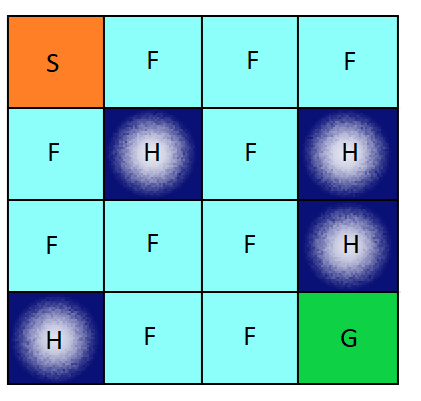
\includegraphics{images/frozen_lake.png}
\caption{Frozen Lake}
\end{figure}

donde S= starting point (safe), F= frozen surface (safe), H=hole (fall
to your doom), G= goal (where the frisbee is located)

(imagen de
https://www.analyticsindiamag.com/openai-gym-frozen-lake-beginners-guide-reinforcement-learning/)

    Descripción del entorno:

Acciones:

\begin{itemize}
\tightlist
\item
  \^{} - Arriba
\item
  v - Abajo
\item
  \textgreater{} - Derecha
\item
  \textless{} - Izquierda
\end{itemize}

Función de recompensa:

\begin{itemize}
\tightlist
\item
  \(+1\) por llegar a estado Goal
\item
  \(0\) en todos los demás estados
\end{itemize}

Función de transición:

\begin{itemize}
\tightlist
\item
  Con el atributo slippery en False cada acción mueve el agente en tal
  sentido con una probabilidad del 100,0\%. Con slippery en True, el
  66,6\% de las veces el agente se moverá a la casilla deseada, mientras
  que el 33,3\% de las veces el agente se moverá a otra posición,
  determinada aleatoriamente.
\end{itemize}

Nota: slippery es un atributo en el entorno FrozenLake que hace que el
hielo sea o no resbaladizo, haciendo que el 33\% de las veces la acción
ejecutada sea aleatoria. En el agente implementado de este notebook el
mismo se desactivó para poder analizar mejor el desempeño del agente.

    \subsubsection{Ejecución de agente aleatorio en
FrozenLake}\label{ejecuciuxf3n-de-agente-aleatorio-en-frozenlake}

    \begin{Verbatim}[commandchars=\\\{\}]
{\color{incolor}In [{\color{incolor}3}]:} \PY{n}{env} \PY{o}{=} \PY{n}{gym}\PY{o}{.}\PY{n}{make}\PY{p}{(}\PY{l+s+s1}{\PYZsq{}}\PY{l+s+s1}{FrozenLake\PYZhy{}v0}\PY{l+s+s1}{\PYZsq{}}\PY{p}{)}
        \PY{n}{env}\PY{o}{.}\PY{n}{reset}\PY{p}{(}\PY{p}{)}
        \PY{k}{for} \PY{n}{\PYZus{}} \PY{o+ow}{in} \PY{n+nb}{range}\PY{p}{(}\PY{l+m+mi}{10}\PY{p}{)}\PY{p}{:}
            \PY{n}{clear\PYZus{}output}\PY{p}{(}\PY{p}{)}
            \PY{n}{env}\PY{o}{.}\PY{n}{render}\PY{p}{(}\PY{p}{)}
            \PY{n}{time}\PY{o}{.}\PY{n}{sleep}\PY{p}{(}\PY{l+m+mi}{1}\PY{p}{)}
            \PY{n}{observation}\PY{p}{,} \PY{n}{reward}\PY{p}{,} \PY{n}{done}\PY{p}{,} \PY{n}{info} \PY{o}{=} \PY{n}{env}\PY{o}{.}\PY{n}{step}\PY{p}{(}\PY{n}{env}\PY{o}{.}\PY{n}{action\PYZus{}space}\PY{o}{.}\PY{n}{sample}\PY{p}{(}\PY{p}{)}\PY{p}{)} \PY{c+c1}{\PYZsh{} se ejecuta una acción aleatoria}
            \PY{k}{if} \PY{n}{done}\PY{p}{:}
                \PY{n}{env}\PY{o}{.}\PY{n}{reset}\PY{p}{(}\PY{p}{)}
        \PY{n}{env}\PY{o}{.}\PY{n}{close}\PY{p}{(}\PY{p}{)}
\end{Verbatim}


    \begin{Verbatim}[commandchars=\\\{\}]
  (Up)
S\setlength{\fboxsep}{0pt}\colorbox{ansi-red}{F\strut}FF
FHFH
FFFH
HFFG

    \end{Verbatim}

    \subsubsection{Configuración básica}\label{configuraciuxf3n-buxe1sica}

    \begin{Verbatim}[commandchars=\\\{\}]
{\color{incolor}In [{\color{incolor}4}]:} \PY{k+kn}{import} \PY{n+nn}{numpy} \PY{k}{as} \PY{n+nn}{np}
        \PY{k+kn}{import} \PY{n+nn}{matplotlib}\PY{n+nn}{.}\PY{n+nn}{pyplot} \PY{k}{as} \PY{n+nn}{plt}
        \PY{k+kn}{from} \PY{n+nn}{agents}\PY{n+nn}{.}\PY{n+nn}{frozen\PYZus{}lake\PYZus{}agent} \PY{k}{import} \PY{n}{FrozenLakeAgent} \PY{k}{as} \PY{n}{fP}
        \PY{k+kn}{import} \PY{n+nn}{itertools}
        
        \PY{c+c1}{\PYZsh{} definimos sus híper\PYZhy{}parámetros básicos}
        
        \PY{n}{alpha} \PY{o}{=} \PY{l+m+mf}{0.5}
        \PY{n}{gamma} \PY{o}{=} \PY{l+m+mf}{0.9}
        \PY{n}{epsilon} \PY{o}{=} \PY{l+m+mf}{0.1}
        \PY{n}{tau} \PY{o}{=} \PY{l+m+mi}{25}
        \PY{n}{is\PYZus{}slippery} \PY{o}{=} \PY{k+kc}{False}
        \PY{n}{cutoff\PYZus{}time} \PY{o}{=} \PY{l+m+mi}{100}  \PY{c+c1}{\PYZsh{} el tiempo de corte del agente son 100 time\PYZhy{}steps, por lo que mantenemos el máximo (es posible bajarlo)}
        
        \PY{c+c1}{\PYZsh{} se declara una semilla aleatoria}
        \PY{n}{random\PYZus{}state} \PY{o}{=} \PY{n}{np}\PY{o}{.}\PY{n}{random}\PY{o}{.}\PY{n}{RandomState}\PY{p}{(}\PY{l+m+mi}{20}\PY{p}{)}
        
        \PY{c+c1}{\PYZsh{} instanciamos nuestro agente}
        \PY{n}{agent} \PY{o}{=} \PY{n}{fP}\PY{o}{.}\PY{n}{FrozenLakeAgent}\PY{p}{(}\PY{p}{)}
        \PY{n}{agent}\PY{o}{.}\PY{n}{random\PYZus{}state} \PY{o}{=} \PY{n}{random\PYZus{}state}
        
        \PY{n}{agent}\PY{o}{.}\PY{n}{set\PYZus{}hyper\PYZus{}parameters}\PY{p}{(}\PY{p}{\PYZob{}}\PY{l+s+s2}{\PYZdq{}}\PY{l+s+s2}{alpha}\PY{l+s+s2}{\PYZdq{}}\PY{p}{:} \PY{n}{alpha}\PY{p}{,} \PY{l+s+s2}{\PYZdq{}}\PY{l+s+s2}{gamma}\PY{l+s+s2}{\PYZdq{}}\PY{p}{:} \PY{n}{gamma}\PY{p}{,} \PY{l+s+s2}{\PYZdq{}}\PY{l+s+s2}{epsilon}\PY{l+s+s2}{\PYZdq{}}\PY{p}{:} \PY{n}{epsilon}\PY{p}{\PYZcb{}}\PY{p}{)}
        
        \PY{c+c1}{\PYZsh{} declaramos como True la variable de mostrar video, para ver en tiempo real cómo aprende el agente. Borrar esta línea}
        \PY{c+c1}{\PYZsh{} para acelerar la velocidad del aprendizaje}
        \PY{n}{agent}\PY{o}{.}\PY{n}{display\PYZus{}video} \PY{o}{=} \PY{k+kc}{True}
        
        \PY{c+c1}{\PYZsh{} establece el tiempo de}
        \PY{n}{agent}\PY{o}{.}\PY{n}{set\PYZus{}cutoff\PYZus{}time}\PY{p}{(}\PY{n}{cutoff\PYZus{}time}\PY{p}{)}
\end{Verbatim}


    \subsubsection{Inicialización y ejecución del
agente}\label{inicializaciuxf3n-y-ejecuciuxf3n-del-agente}

    \begin{Verbatim}[commandchars=\\\{\}]
{\color{incolor}In [{\color{incolor}5}]:} \PY{c+c1}{\PYZsh{} inicializa el agente}
        \PY{n}{agent}\PY{o}{.}\PY{n}{init\PYZus{}agent}\PY{p}{(}\PY{n}{is\PYZus{}slippery}\PY{o}{=}\PY{n}{is\PYZus{}slippery}\PY{p}{)}  \PY{c+c1}{\PYZsh{} slippery es establecido en False por defecto}
        
        \PY{c+c1}{\PYZsh{} reinicializa el conocimiento del agente}
        \PY{n}{agent}\PY{o}{.}\PY{n}{restart\PYZus{}agent\PYZus{}learning}\PY{p}{(}\PY{p}{)}
        
        \PY{c+c1}{\PYZsh{} se realiza la ejecución del agente}
        \PY{n}{avg\PYZus{}steps\PYZus{}per\PYZus{}episode} \PY{o}{=} \PY{n}{agent}\PY{o}{.}\PY{n}{run}\PY{p}{(}\PY{p}{)}
\end{Verbatim}


    \subsubsection{Análisis de la ejecución del
agente}\label{anuxe1lisis-de-la-ejecuciuxf3n-del-agente}

\paragraph{Análisis de convergencia}\label{anuxe1lisis-de-convergencia}

A diferencia de lo que sucede en el aprendizaje supervisado, en el
aprendizaje por refuerzos el rendimiento se evalúa por una función
específica que es la función de recompensa. En la práctica, la función
de recompensa puede ser externa (y provista por el entorno) o bien puede
ser una función creada por diseño (a modo de dirigir el agente hacia lo
que por diseño se considera mejor, en nuestro ejemplo podría ser con una
recompensa de \(-1\) cada vez que el agente llega a un estado H) o bien
combinar ambos enfoques (usando recompensas obtenidas desde el entorno y
generadas por diseño).

Como el objetivo de RL es maximizar la recompensa obtenida, es posible
utilizar la información sobre la obtención de la recompensas en cada
time-step o episodio para evaluar el rendimiento parcial del agente
(esto depende mucho de la particularidad de la distribución de la
recompensa para el problema tratado).

    Para analizar la ejecución del agente, vamos a ver cómo se desempeñó el
mismo en dos aspectos:

\begin{itemize}
\item
  Recompensa obtenida en cada episodio: nos dirá cuánta recompensa
  obtuvo el agente en cada uno de los episodios. Con esta medida
  sabremos al instante si el agente pudo llegar al estado Goal en cada
  uno de los episodios, habiendo recibido una recompensa de \(1\), donde
  en caso contrario habrá recibido una recompensa de \(0\).
\item
  Pasos transcurridos en cada episodio: indicará cuántos pasos le ha
  llevado al agente la ejecución del episodio. Si bien este indicador no
  garantiza que el agente haya llegado al estado G, indicará cómo el
  mismo tiende a realizar su aprendizaje (si aprende debería tender a
  bajar la cantidad de pasos por cada episodio).
\end{itemize}

    Veamos recompensa por episodio (recordar que en este entorno cada paso
otorga una recompensa de \(0\) excepto en aquellos en los que se arriba
al estado Goal, donde la recompensa es de \(1\))

    \begin{Verbatim}[commandchars=\\\{\}]
{\color{incolor}In [{\color{incolor}6}]:} \PY{n}{episode\PYZus{}rewards} \PY{o}{=} \PY{n}{np}\PY{o}{.}\PY{n}{array}\PY{p}{(}\PY{n}{agent}\PY{o}{.}\PY{n}{reward\PYZus{}of\PYZus{}episode}\PY{p}{)}
        \PY{n}{plt}\PY{o}{.}\PY{n}{scatter}\PY{p}{(}\PY{n}{np}\PY{o}{.}\PY{n}{array}\PY{p}{(}\PY{n+nb}{range}\PY{p}{(}\PY{l+m+mi}{0}\PY{p}{,} \PY{n+nb}{len}\PY{p}{(}\PY{n}{episode\PYZus{}rewards}\PY{p}{)}\PY{p}{)}\PY{p}{)}\PY{p}{,} \PY{n}{episode\PYZus{}rewards}\PY{p}{,} \PY{n}{s}\PY{o}{=}\PY{l+m+mf}{0.7}\PY{p}{)}
        \PY{n}{plt}\PY{o}{.}\PY{n}{title}\PY{p}{(}\PY{l+s+s1}{\PYZsq{}}\PY{l+s+s1}{Recompensa por episodio}\PY{l+s+s1}{\PYZsq{}}\PY{p}{)}
        \PY{n}{plt}\PY{o}{.}\PY{n}{show}\PY{p}{(}\PY{p}{)}
\end{Verbatim}


    \begin{center}
    \adjustimage{max size={0.9\linewidth}{0.9\paperheight}}{output_20_0.png}
    \end{center}
    { \hspace*{\fill} \\}
    
    Veamos pasos por episodio

    \begin{Verbatim}[commandchars=\\\{\}]
{\color{incolor}In [{\color{incolor}7}]:} \PY{c+c1}{\PYZsh{} se muestra la curva de aprendizaje de los pasos por episodio}
        \PY{n}{episode\PYZus{}steps} \PY{o}{=} \PY{n}{np}\PY{o}{.}\PY{n}{array}\PY{p}{(}\PY{n}{agent}\PY{o}{.}\PY{n}{timesteps\PYZus{}of\PYZus{}episode}\PY{p}{)}
        \PY{n}{plt}\PY{o}{.}\PY{n}{plot}\PY{p}{(}\PY{n}{np}\PY{o}{.}\PY{n}{array}\PY{p}{(}\PY{n+nb}{range}\PY{p}{(}\PY{l+m+mi}{0}\PY{p}{,} \PY{n+nb}{len}\PY{p}{(}\PY{n}{episode\PYZus{}steps}\PY{p}{)}\PY{p}{)}\PY{p}{)}\PY{p}{,} \PY{n}{episode\PYZus{}steps}\PY{p}{)}
        \PY{n}{plt}\PY{o}{.}\PY{n}{title}\PY{p}{(}\PY{l+s+s1}{\PYZsq{}}\PY{l+s+s1}{Pasos (timesteps) por episodio}\PY{l+s+s1}{\PYZsq{}}\PY{p}{)}
        \PY{n}{plt}\PY{o}{.}\PY{n}{show}\PY{p}{(}\PY{p}{)}
\end{Verbatim}


    \begin{center}
    \adjustimage{max size={0.9\linewidth}{0.9\paperheight}}{output_22_0.png}
    \end{center}
    { \hspace*{\fill} \\}
    
    Como vemos, los gráficos arrojan algo de información pero a su vez
oscilan demasiado. Para contrarrestar esto procedemos a suavizarlos:

    \begin{Verbatim}[commandchars=\\\{\}]
{\color{incolor}In [{\color{incolor}8}]:} \PY{c+c1}{\PYZsh{} se suaviza la curva de convergencia}
        \PY{n}{episode\PYZus{}number} \PY{o}{=} \PY{n}{np}\PY{o}{.}\PY{n}{linspace}\PY{p}{(}\PY{l+m+mi}{1}\PY{p}{,} \PY{n+nb}{len}\PY{p}{(}\PY{n}{episode\PYZus{}rewards}\PY{p}{)} \PY{o}{+} \PY{l+m+mi}{1}\PY{p}{,} \PY{n+nb}{len}\PY{p}{(}\PY{n}{episode\PYZus{}rewards}\PY{p}{)} \PY{o}{+} \PY{l+m+mi}{1}\PY{p}{)}
        \PY{n}{acumulated\PYZus{}rewards} \PY{o}{=} \PY{n}{np}\PY{o}{.}\PY{n}{cumsum}\PY{p}{(}\PY{n}{episode\PYZus{}rewards}\PY{p}{)}
        
        \PY{n}{reward\PYZus{}per\PYZus{}episode} \PY{o}{=} \PY{p}{[}\PY{n}{acumulated\PYZus{}rewards}\PY{p}{[}\PY{n}{i}\PY{p}{]} \PY{o}{/} \PY{n}{episode\PYZus{}number}\PY{p}{[}\PY{n}{i}\PY{p}{]} \PY{k}{for} \PY{n}{i} \PY{o+ow}{in} \PY{n+nb}{range}\PY{p}{(}\PY{n+nb}{len}\PY{p}{(}\PY{n}{acumulated\PYZus{}rewards}\PY{p}{)}\PY{p}{)}\PY{p}{]}
        
        \PY{n}{plt}\PY{o}{.}\PY{n}{plot}\PY{p}{(}\PY{n}{reward\PYZus{}per\PYZus{}episode}\PY{p}{)}
        \PY{n}{plt}\PY{o}{.}\PY{n}{title}\PY{p}{(}\PY{l+s+s1}{\PYZsq{}}\PY{l+s+s1}{Recompensa acumulada por episodio}\PY{l+s+s1}{\PYZsq{}}\PY{p}{)}
        \PY{n}{plt}\PY{o}{.}\PY{n}{show}\PY{p}{(}\PY{p}{)}
\end{Verbatim}


    \begin{center}
    \adjustimage{max size={0.9\linewidth}{0.9\paperheight}}{output_24_0.png}
    \end{center}
    { \hspace*{\fill} \\}
    
    \begin{Verbatim}[commandchars=\\\{\}]
{\color{incolor}In [{\color{incolor}9}]:} \PY{c+c1}{\PYZsh{} se suaviza la curva de aprendizaje}
        \PY{n}{episode\PYZus{}number} \PY{o}{=} \PY{n}{np}\PY{o}{.}\PY{n}{linspace}\PY{p}{(}\PY{l+m+mi}{1}\PY{p}{,} \PY{n+nb}{len}\PY{p}{(}\PY{n}{episode\PYZus{}steps}\PY{p}{)} \PY{o}{+} \PY{l+m+mi}{1}\PY{p}{,} \PY{n+nb}{len}\PY{p}{(}\PY{n}{episode\PYZus{}steps}\PY{p}{)} \PY{o}{+} \PY{l+m+mi}{1}\PY{p}{)}
        \PY{n}{acumulated\PYZus{}steps} \PY{o}{=} \PY{n}{np}\PY{o}{.}\PY{n}{cumsum}\PY{p}{(}\PY{n}{episode\PYZus{}steps}\PY{p}{)}
        
        \PY{n}{steps\PYZus{}per\PYZus{}episode} \PY{o}{=} \PY{p}{[}\PY{n}{acumulated\PYZus{}steps}\PY{p}{[}\PY{n}{i}\PY{p}{]} \PY{o}{/} \PY{n}{episode\PYZus{}number}\PY{p}{[}\PY{n}{i}\PY{p}{]} \PY{k}{for} \PY{n}{i} \PY{o+ow}{in} \PY{n+nb}{range}\PY{p}{(}\PY{n+nb}{len}\PY{p}{(}\PY{n}{acumulated\PYZus{}steps}\PY{p}{)}\PY{p}{)}\PY{p}{]}
        
        \PY{n}{plt}\PY{o}{.}\PY{n}{plot}\PY{p}{(}\PY{n}{steps\PYZus{}per\PYZus{}episode}\PY{p}{)}
        \PY{n}{plt}\PY{o}{.}\PY{n}{title}\PY{p}{(}\PY{l+s+s1}{\PYZsq{}}\PY{l+s+s1}{Pasos (timesteps) acumulados por episodio}\PY{l+s+s1}{\PYZsq{}}\PY{p}{)}
        \PY{n}{plt}\PY{o}{.}\PY{n}{show}\PY{p}{(}\PY{p}{)}
\end{Verbatim}


    \begin{center}
    \adjustimage{max size={0.9\linewidth}{0.9\paperheight}}{output_25_0.png}
    \end{center}
    { \hspace*{\fill} \\}
    
    \paragraph{Análisis de matriz de valor y política
óptima}\label{anuxe1lisis-de-matriz-de-valor-y-poluxedtica-uxf3ptima}

Siendo que este es un ejemplo tabular y de pocos estados / acciones, es
posible realizar un análisis de convergencia desde otro punto de vista:
desde el valor que alcanzó cada estado al finalizar la ejecución del
agente y la acción que ejecutaría al llegar a cada estado*. Ambos nos
brindarán información sobre la convergencia alcanzada por el agente.

Teniendo los valores de \(Q(s,a)\) para cada par estado-acción, el valor
de cada estado se calcula a través de

\[V(s) = \sum_{a} \pi(a \mid s) Q(s, a) \]

donde \(\pi(a \mid s)\) es la probabilidad de tomar la acción \(a\)
siendo que el agente se encuentra en el estado \(s\). Siguiendo la
política \(\epsilon\)-greedy, donde como ejemplo \(\epsilon = 0.25\) y
dado el conjunto de acciones posibles \(A\) donde \(\mid\;A\mid=4\),
\(\pi(a \mid s)\) está dado por:

\[ \pi(a \mid s) = \begin{cases}
                        0.75 + \frac{0.25}{4} & \text{si $a$ es la mejor acción}\\
                        \frac{0.25}{4} & \text{en caso contrario}
                   \end{cases}
\]

Notar que la fracción \(\frac{0.25}{4}\) se añade pues se tiene en
cuenta que \(a\) puede haber sido elegida aleatoriamente al ejecutar una
acción exploratoria. Un criterio distinto podría ser que en la acción
exploratoria se excluya a la mejor acción.

(*) Tener en cuenta que este análisis se hace principalmente con fines
educativos, para entornos más complejos el mismo puede no ser factible.
En tales casos, un análisis alternativo podría consistir en hacer que el
agente ejecute su política para la que fue entrenado, para hacer una
evaluación a partir del comportamiento del mismo.

    Por otra parte, la acción óptima para cada estado se obtiene simplemente
consultando el \(Q(s,a)\) que mayor valor arroja. Gráficamente:

    \begin{Verbatim}[commandchars=\\\{\}]
{\color{incolor}In [{\color{incolor}10}]:} \PY{c+c1}{\PYZsh{} se procede con los cálculos previos a la graficación de la matriz de valor}
         \PY{n}{value\PYZus{}matrix} \PY{o}{=} \PY{n}{np}\PY{o}{.}\PY{n}{zeros}\PY{p}{(}\PY{p}{(}\PY{l+m+mi}{4}\PY{p}{,} \PY{l+m+mi}{4}\PY{p}{)}\PY{p}{)}
         \PY{k}{for} \PY{n}{row} \PY{o+ow}{in} \PY{n+nb}{range}\PY{p}{(}\PY{l+m+mi}{4}\PY{p}{)}\PY{p}{:}
             \PY{k}{for} \PY{n}{column} \PY{o+ow}{in} \PY{n+nb}{range}\PY{p}{(}\PY{l+m+mi}{4}\PY{p}{)}\PY{p}{:}
         
                 \PY{n}{state\PYZus{}values} \PY{o}{=} \PY{p}{[}\PY{p}{]}
         
                 \PY{k}{for} \PY{n}{action} \PY{o+ow}{in} \PY{n+nb}{range}\PY{p}{(}\PY{l+m+mi}{4}\PY{p}{)}\PY{p}{:}
                     \PY{n}{state\PYZus{}values}\PY{o}{.}\PY{n}{append}\PY{p}{(}\PY{n}{agent}\PY{o}{.}\PY{n}{q}\PY{o}{.}\PY{n}{get}\PY{p}{(}\PY{p}{(}\PY{n}{row} \PY{o}{*} \PY{l+m+mi}{4} \PY{o}{+} \PY{n}{column}\PY{p}{,} \PY{n}{action}\PY{p}{)}\PY{p}{,} \PY{l+m+mi}{0}\PY{p}{)}\PY{p}{)}
                     
                 \PY{n+nb}{print}\PY{p}{(}\PY{n}{state\PYZus{}values}\PY{p}{)}
         
                 \PY{n}{maximum\PYZus{}value} \PY{o}{=} \PY{n+nb}{max}\PY{p}{(}\PY{n}{state\PYZus{}values}\PY{p}{)}  \PY{c+c1}{\PYZsh{} como usamos epsilon\PYZhy{}greedy, determinamos la acción que arroja máximo valor}
                 \PY{n}{state\PYZus{}values}\PY{o}{.}\PY{n}{remove}\PY{p}{(}\PY{n}{maximum\PYZus{}value}\PY{p}{)}  \PY{c+c1}{\PYZsh{} removemos el ítem asociado con la acción de máximo valor}
                 
                 \PY{c+c1}{\PYZsh{} el valor de la matriz para la mejor acción es el máximo valor por la probabilidad de que el mismo sea elegido}
                 \PY{c+c1}{\PYZsh{} (que es 1\PYZhy{}epsilon por la probabilidad de explotación más 1/4 * epsilon por probabilidad de que sea elegido al}
                 \PY{c+c1}{\PYZsh{} azar cuando se opta por una acción exploratoria)}
                 \PY{n}{value\PYZus{}matrix}\PY{p}{[}\PY{n}{row}\PY{p}{,} \PY{n}{column}\PY{p}{]} \PY{o}{=} \PY{n}{maximum\PYZus{}value} \PY{o}{*} \PY{p}{(}\PY{l+m+mi}{1} \PY{o}{\PYZhy{}} \PY{n}{epsilon} \PY{o}{+} \PY{p}{(}\PY{l+m+mi}{1}\PY{o}{/}\PY{l+m+mi}{4} \PY{o}{*} \PY{n}{epsilon}\PY{p}{)}\PY{p}{)}
                 
                 \PY{k}{for} \PY{n}{non\PYZus{}maximum\PYZus{}value} \PY{o+ow}{in} \PY{n}{state\PYZus{}values}\PY{p}{:}
                     \PY{c+c1}{\PYZsh{}value\PYZus{}matrix[row, column] += (epsilon/4) * non\PYZus{}maximum\PYZus{}value}
                     \PY{n}{value\PYZus{}matrix}\PY{p}{[}\PY{n}{row}\PY{p}{,} \PY{n}{column}\PY{p}{]} \PY{o}{+}\PY{o}{=} \PY{p}{(}\PY{l+m+mi}{1} \PY{o}{\PYZhy{}} \PY{p}{(}\PY{l+m+mi}{1} \PY{o}{\PYZhy{}} \PY{n}{epsilon} \PY{o}{+} \PY{p}{(}\PY{l+m+mi}{1}\PY{o}{/}\PY{l+m+mi}{4} \PY{o}{*} \PY{n}{epsilon}\PY{p}{)}\PY{p}{)}\PY{p}{)}\PY{o}{/}\PY{l+m+mi}{3} \PY{o}{*} \PY{n}{non\PYZus{}maximum\PYZus{}value}
         
         \PY{c+c1}{\PYZsh{} el valor del estado objetivo se asigna en 1 (reward recibido al llegar) para que se coloree de forma apropiada}
         \PY{n}{value\PYZus{}matrix}\PY{p}{[}\PY{l+m+mi}{3}\PY{p}{,} \PY{l+m+mi}{3}\PY{p}{]} \PY{o}{=} \PY{l+m+mi}{1}
         
         \PY{c+c1}{\PYZsh{} se grafica la matriz de valor}
         \PY{n}{plt}\PY{o}{.}\PY{n}{imshow}\PY{p}{(}\PY{n}{value\PYZus{}matrix}\PY{p}{,} \PY{n}{cmap}\PY{o}{=}\PY{n}{plt}\PY{o}{.}\PY{n}{cm}\PY{o}{.}\PY{n}{RdYlGn}\PY{p}{)}
         \PY{n}{plt}\PY{o}{.}\PY{n}{tight\PYZus{}layout}\PY{p}{(}\PY{p}{)}
         \PY{n}{plt}\PY{o}{.}\PY{n}{colorbar}\PY{p}{(}\PY{p}{)}
         
         \PY{n}{fmt} \PY{o}{=} \PY{l+s+s1}{\PYZsq{}}\PY{l+s+s1}{.2f}\PY{l+s+s1}{\PYZsq{}}
         \PY{n}{thresh} \PY{o}{=} \PY{n}{value\PYZus{}matrix}\PY{o}{.}\PY{n}{max}\PY{p}{(}\PY{p}{)} \PY{o}{/} \PY{l+m+mf}{2.}
         \PY{k}{for} \PY{n}{row}\PY{p}{,} \PY{n}{column} \PY{o+ow}{in} \PY{n}{itertools}\PY{o}{.}\PY{n}{product}\PY{p}{(}\PY{n+nb}{range}\PY{p}{(}\PY{n}{value\PYZus{}matrix}\PY{o}{.}\PY{n}{shape}\PY{p}{[}\PY{l+m+mi}{0}\PY{p}{]}\PY{p}{)}\PY{p}{,} \PY{n+nb}{range}\PY{p}{(}\PY{n}{value\PYZus{}matrix}\PY{o}{.}\PY{n}{shape}\PY{p}{[}\PY{l+m+mi}{1}\PY{p}{]}\PY{p}{)}\PY{p}{)}\PY{p}{:}
         
             \PY{n}{left\PYZus{}action} \PY{o}{=} \PY{n}{agent}\PY{o}{.}\PY{n}{q}\PY{o}{.}\PY{n}{get}\PY{p}{(}\PY{p}{(}\PY{n}{row} \PY{o}{*} \PY{l+m+mi}{4} \PY{o}{+} \PY{n}{column}\PY{p}{,} \PY{l+m+mi}{0}\PY{p}{)}\PY{p}{,} \PY{l+m+mi}{0}\PY{p}{)}
             \PY{n}{down\PYZus{}action} \PY{o}{=} \PY{n}{agent}\PY{o}{.}\PY{n}{q}\PY{o}{.}\PY{n}{get}\PY{p}{(}\PY{p}{(}\PY{n}{row} \PY{o}{*} \PY{l+m+mi}{4} \PY{o}{+} \PY{n}{column}\PY{p}{,} \PY{l+m+mi}{1}\PY{p}{)}\PY{p}{,} \PY{l+m+mi}{0}\PY{p}{)}
             \PY{n}{right\PYZus{}action} \PY{o}{=} \PY{n}{agent}\PY{o}{.}\PY{n}{q}\PY{o}{.}\PY{n}{get}\PY{p}{(}\PY{p}{(}\PY{n}{row} \PY{o}{*} \PY{l+m+mi}{4} \PY{o}{+} \PY{n}{column}\PY{p}{,} \PY{l+m+mi}{2}\PY{p}{)}\PY{p}{,} \PY{l+m+mi}{0}\PY{p}{)}
             \PY{n}{up\PYZus{}action} \PY{o}{=} \PY{n}{agent}\PY{o}{.}\PY{n}{q}\PY{o}{.}\PY{n}{get}\PY{p}{(}\PY{p}{(}\PY{n}{row} \PY{o}{*} \PY{l+m+mi}{4} \PY{o}{+} \PY{n}{column}\PY{p}{,} \PY{l+m+mi}{3}\PY{p}{)}\PY{p}{,} \PY{l+m+mi}{0}\PY{p}{)}
             
             \PY{n}{arrow\PYZus{}direction} \PY{o}{=} \PY{l+s+s1}{\PYZsq{}}\PY{l+s+s1}{↓}\PY{l+s+s1}{\PYZsq{}}
             \PY{n}{best\PYZus{}action} \PY{o}{=} \PY{n}{down\PYZus{}action}
             
             \PY{k}{if} \PY{n}{best\PYZus{}action} \PY{o}{\PYZlt{}} \PY{n}{right\PYZus{}action}\PY{p}{:}
                 \PY{n}{arrow\PYZus{}direction} \PY{o}{=} \PY{l+s+s1}{\PYZsq{}}\PY{l+s+s1}{→}\PY{l+s+s1}{\PYZsq{}}
                 \PY{n}{best\PYZus{}action} \PY{o}{=} \PY{n}{right\PYZus{}action}
             \PY{k}{if} \PY{n}{best\PYZus{}action} \PY{o}{\PYZlt{}} \PY{n}{left\PYZus{}action}\PY{p}{:}
                 \PY{n}{arrow\PYZus{}direction} \PY{o}{=} \PY{l+s+s1}{\PYZsq{}}\PY{l+s+s1}{←}\PY{l+s+s1}{\PYZsq{}}
                 \PY{n}{best\PYZus{}action} \PY{o}{=} \PY{n}{left\PYZus{}action}
             \PY{k}{if} \PY{n}{best\PYZus{}action} \PY{o}{\PYZlt{}} \PY{n}{up\PYZus{}action}\PY{p}{:}
                 \PY{n}{arrow\PYZus{}direction} \PY{o}{=} \PY{l+s+s1}{\PYZsq{}}\PY{l+s+s1}{↑}\PY{l+s+s1}{\PYZsq{}}
                 \PY{n}{best\PYZus{}action} \PY{o}{=} \PY{n}{up\PYZus{}action}
             \PY{k}{if} \PY{n}{best\PYZus{}action} \PY{o}{==} \PY{l+m+mi}{0}\PY{p}{:}
                 \PY{n}{arrow\PYZus{}direction} \PY{o}{=} \PY{l+s+s1}{\PYZsq{}}\PY{l+s+s1}{\PYZsq{}}
             \PY{n+nb}{print}\PY{p}{(}\PY{n}{left\PYZus{}action}\PY{p}{,} \PY{n}{down\PYZus{}action}\PY{p}{,} \PY{n}{right\PYZus{}action}\PY{p}{,} \PY{n}{up\PYZus{}action}\PY{p}{,} \PY{n}{column}\PY{p}{,} \PY{n}{row}\PY{p}{)}
             \PY{c+c1}{\PYZsh{} notar que column, row están invertidos en orden en la línea de abajo porque representan a x,y del plot}
             \PY{n}{plt}\PY{o}{.}\PY{n}{text}\PY{p}{(}\PY{n}{column}\PY{p}{,} \PY{n}{row}\PY{p}{,} \PY{n}{arrow\PYZus{}direction}\PY{p}{,}
                      \PY{n}{horizontalalignment}\PY{o}{=}\PY{l+s+s2}{\PYZdq{}}\PY{l+s+s2}{center}\PY{l+s+s2}{\PYZdq{}}\PY{p}{)}
         
         \PY{n}{plt}\PY{o}{.}\PY{n}{xticks}\PY{p}{(}\PY{p}{[}\PY{p}{]}\PY{p}{)}
         \PY{n}{plt}\PY{o}{.}\PY{n}{yticks}\PY{p}{(}\PY{p}{[}\PY{p}{]}\PY{p}{)}
         \PY{n}{plt}\PY{o}{.}\PY{n}{show}\PY{p}{(}\PY{p}{)}
         
         \PY{n+nb}{print}\PY{p}{(}\PY{l+s+s1}{\PYZsq{}}\PY{l+s+se}{\PYZbs{}n}\PY{l+s+s1}{ Matriz de valor (en números): }\PY{l+s+se}{\PYZbs{}n}\PY{l+s+se}{\PYZbs{}n}\PY{l+s+s1}{\PYZsq{}}\PY{p}{,} \PY{n}{value\PYZus{}matrix}\PY{p}{)}
\end{Verbatim}


    \begin{Verbatim}[commandchars=\\\{\}]
[0.5314409999999998, 0.59049, 0.4782968999999998, 0.5314409999999998]
[0.5314409999999998, 0.0, 0.3280499999236153, 0.4184513918537383]
[0.0, 0.6834374999787806, 0.0, 0.0]
[0.0, 0.0, 0.0, 0.0]
[0.59049, 0.6560999999999999, 0.0, 0.5314409999999998]
[0, 0, 0, 0]
[0.0, 0.8099999999999998, 0.0, 0.2870437499809026]
[0, 0, 0, 0]
[0.6560999999999999, 0.0, 0.7289999999999999, 0.59049]
[0.6560999999999999, 0.8099999999999998, 0.8099999999999998, 0.0]
[0.7289999999999999, 0.8999999999999999, 0.0, 0.728999999999999]
[0, 0, 0, 0]
[0, 0, 0, 0]
[0.0, 0.8096044921874308, 0.8999999999999999, 0.7289110107421873]
[0.8099999999999998, 0.8999999999999999, 1.0, 0.8099999999999998]
[0, 0, 0, 0]
0.5314409999999998 0.59049 0.4782968999999998 0.5314409999999998 0 0
0.5314409999999998 0.0 0.3280499999236153 0.4184513918537383 1 0
0.0 0.6834374999787806 0.0 0.0 2 0
0.0 0.0 0.0 0.0 3 0
0.59049 0.6560999999999999 0.0 0.5314409999999998 0 1
0 0 0 0 1 1
0.0 0.8099999999999998 0.0 0.2870437499809026 2 1
0 0 0 0 3 1
0.6560999999999999 0.0 0.7289999999999999 0.59049 0 2
0.6560999999999999 0.8099999999999998 0.8099999999999998 0.0 1 2
0.7289999999999999 0.8999999999999999 0.0 0.728999999999999 2 2
0 0 0 0 3 2
0 0 0 0 0 3
0.0 0.8096044921874308 0.8999999999999999 0.7289110107421873 1 3
0.8099999999999998 0.8999999999999999 1.0 0.8099999999999998 2 3
0 0 0 0 3 3

    \end{Verbatim}

    \begin{center}
    \adjustimage{max size={0.9\linewidth}{0.9\paperheight}}{output_28_1.png}
    \end{center}
    { \hspace*{\fill} \\}
    
    \begin{Verbatim}[commandchars=\\\{\}]

 Matriz de valor (en números): 

 [[0.58473272 0.51024546 0.63217969 0.        ]
 [0.63494077 0.         0.75642609 0.        ]
 [0.70548975 0.7859025  0.86895    0.        ]
 [0.         0.87096289 0.988      1.        ]]

    \end{Verbatim}

    \begin{Verbatim}[commandchars=\\\{\}]
{\color{incolor}In [{\color{incolor}11}]:} \PY{c+c1}{\PYZsh{} destrucción del agente}
         \PY{n}{agent}\PY{o}{.}\PY{n}{destroy\PYZus{}agent}\PY{p}{(}\PY{p}{)}
\end{Verbatim}


    \subsection{Ejercicios Lab1}\label{ejercicios-lab1}

Para el presente trabajo práctico vamos a utilizar las clases
FrozenLakeAgent y QLearning (tabular), llamadas desde el presente
notebook, y el script \emph{frozenlake\_main\_script}, ubicado en
\emph{agents/frozen\_lake\_agent/}. Tales scripts se presentan como
herramientas para resolver los ejercicios, por lo se permite, para la
resolución de los mismos, modificarlos o reemplazarlos por sus propias
implementaciones. Cada uno presenta la siguiente funcionalidad:

\begin{quote}
frozenlake\_main\_script
\end{quote}

Script que crea y define la configuración inicial del agente de RL de
tipo FrozenLake, creando la instancia de FrozenLakeAgent.

\begin{quote}
FrozenLakeAgent
\end{quote}

Clase que implementa la interfaz con OpenAIGym, creando el entorno e
iterando el mismo. Adicionalmente provee una interfaz para llamar y
correr el agente RL.

\begin{quote}
QLearning
\end{quote}

Clase que implementa el algoritmo QLearning, lo cual involucra el
guardado de los valores de Q en un diccionario, la selección de acciones
(mediante \(choose\_action\)) y la actualización de los valores de Q
(mediante \(learn\)).

\textbf{Recomendación}: No se sugiere hacer este TP desde jupyter
notebook/lab sino desde un IDE estilo Pycharm, debido a que los
algoritmos de RL suelen requerir un debug paso a paso, tanto para
corregir errores como para entender mejor cómo funcionan los mismos.

Se pide:

\begin{enumerate}
\def\labelenumi{\arabic{enumi}.}
\item
  Dado el agente de Q-Learning en el entorno FrozenLake, implementar la
  política Softmax, dada por
  \[\pi(a \mid s) = \frac{e^{Q(s,a)/\tau}}{\sum_{a'}e^{Q(s,a')/\tau}}\]
\item
  Realizar una breve descripción analizando cómo difieren en la curva de
  aprendizaje los distintos valores de los híper-parámetros \(\alpha\),
  \(\epsilon\), \(\tau\) y \(\gamma\) tanto con política
  \(\epsilon\)-greedy como con Softmax.
\item
  Implementar algoritmo SARSA y compararlo con Q-Learning, en la curva
  de convergencia de la recompensa. (Opcional) compararlos también en la
  matriz de valor, para lo cuál debe adaptarse la matriz de valor a la
  política Softmax (actualmente la misma está de acuerdo a la política
  epsilon-greedy).
\item
  Evaluar evaluar cómo cambia el desempeño de los algoritmos
  implementados con el entorno FrozenLake con Slippery = True. ¿Cómo se
  comparan Q-Learning y SARSA? ¿Cómo es esta comparación de acuerdo a
  sus híper-parámetros?
\item
  (Opcional) Implementar algoritmo Q(\(\lambda\)) y evaluar cómo cambia
  la convergencia con respecto a Q.
\end{enumerate}


    % Add a bibliography block to the postdoc
    
    
    
    \end{document}
